% MA4128

% https://www3.nd.edu/~rwilliam/stats1/OLS-SPSS.pdf
%http://psychweb.psy.umt.edu/denis/datadecision/front/stat_II_2011/psyx_521_multiple_regression_part_II.pdf

% ftp://public.dhe.ibm.com/software/analytics/spss/documentation/statistics/20.0/en/client/Manuals/IBM_SPSS_Regression.pdf

%http://www.education.umd.edu/EDMS/fac/Harring/Past-Classes/EDMS651/Notes/LRA-3.pdf

% http://www.psych.yorku.ca/lab/psy6140/lectures/ModelSelection2x2.pdf

%http://philosophy.wisc.edu/forster/220/simplicity.html

%http://statistics.uchicago.edu/~s220e/Lect/lec21.pdf

%http://publib.boulder.ibm.com/infocenter/spssstat/v20r0m0/index.jsp?topic=%2Fcom.ibm.spss.statistics.help%2Fsyn_regression_criteria_variable_selection.htm

\documentclass[a4paper,12pt]{article}
%%%%%%%%%%%%%%%%%%%%%%%%%%%%%%%%%%%%%%%%%%%%%%%%%%%%%%%%%%%%%%%%%%%%%%%%%%%%%%%%%%%%%%%%%%%%%%%%%%%%%%%%%%%%%%%%%%%%%%%%%%%%%%%%%%%%%%%%%%%%%%%%%%%%%%%%%%%%%%%%%%%%%%%%%%%%%%%%%%%%%%%%%%%%%%%%%%%%%%%%%%%%%%%%%%%%%%%%%%%%%%%%%%%%%%%%%%%%%%%%%%%%%%%%%%%%
\usepackage{eurosym}
\usepackage{vmargin}
\usepackage{amsmath}
\usepackage{graphics}
\usepackage{epsfig}
\usepackage{framed}
\usepackage{subfigure}
\usepackage{fancyhdr}

\setcounter{MaxMatrixCols}{10}
%TCIDATA{OutputFilter=LATEX.DLL}
%TCIDATA{Version=5.00.0.2570}
%TCIDATA{<META NAME="SaveForMode"CONTENT="1">}
%TCIDATA{LastRevised=Wednesday, February 23, 201113:24:34}
%TCIDATA{<META NAME="GraphicsSave" CONTENT="32">}
%TCIDATA{Language=American English}

\pagestyle{fancy}
\setmarginsrb{20mm}{0mm}{20mm}{25mm}{12mm}{11mm}{0mm}{11mm}
\lhead{MA4128} \rhead{Kevin O'Brien} \chead{Week 8} %\input{tcilatex}

%http://www.electronics.dit.ie/staff/ysemenova/Opto2/CO_IntroLab.pdf
\begin{document}

\tableofcontents
\newpage
\section{SLR Example}


The data give the yields of cotton and irrigation levels in the Salt River Valley for different plots of land. Each plot was on Maricopa sandy loam soil. The variables are as follows:
\begin{itemize}
\item \textbf{Irrigation} The amount of irrigation water applied in feet per acre. This is the predictor variable.
\item \textbf{Yield} The yield of Pima cotton in pounds per acre. This is the response variable.
\end{itemize}
\begin{center}
\begin{tabular}{|c|c|c||c|c|c|}
  \hline
  % after \\: \hline or \cline{col1-col2} \cline{col3-col4} ...
  Observation & Irrigation & Yield & Observation & Irrigation & Yield \\\hline
  1 & 1.8	& 260 & 8  &  1.5	& 280 \\
  2 & 1.9	& 370 & 9  & 1.5	& 230 \\
  3 & 2.5	& 450 & 10 & 1.2	& 180 \\
  4 & 1.4	& 160 & 11 & 1.3	& 220 \\
  5 & 1.3	& 90  & 12 & 1.8	& 180 \\
  6 & 2.1	& 440 & 13 & 3.5	& 400 \\
  7 & 2.3	& 380 & 14 & 3.5	& 650 \\
  \hline
\end{tabular}
\end{center}


%\begin{figure}[h!]
%\begin{center}
%  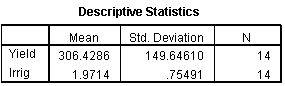
\includegraphics[scale=0.8]{SLR1.png}
%  \caption{SPSS output.}\label{SLR1}
%\end{center}
%\end{figure}


\begin{center}
\begin{table}[htbp]
  \centering
  \caption{Add caption}
    \begin{tabular}{|rrrr|}
    %\toprule
    \hline
    \multicolumn{4}{c}{Descriptive Statistics}  \\
    \hline % midrule
          & \multicolumn{1}{|c|}{Mean} & \multicolumn{1}{|c|}{Std. Deviation} & \multicolumn{1}{|c|}{N} \\
    \multicolumn{1}{|l|}{Yield} & 306.4286 & 149.6461 & 14 \\
    \multicolumn{1}{|l|}{Irrig} & 1.971429 & 0.754911 & 14 \\
    %\bottomrule
    \hline
    \end{tabular}%

\end{table}%
\end{center}

Next we are given the output from the correlation analysis and the regression ANOVA.

%\begin{figure}[h!]
%\begin{center}
%  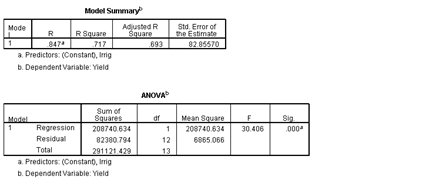
\includegraphics[width=160mm]{SLR3.jpg}
%  \caption{SPSS output.}\label{SLR1}
%\end{center}
%\end{figure}

The intercept and slope estimate are determined by examining the ``coefficients".
%\begin{figure}[h!]
%\begin{center}
%  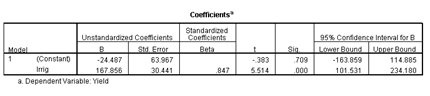
\includegraphics[width=150mm]{SLR2.jpg}
%  \caption{SPSS output.}\label{SLR1}
%\end{center}
%\end{figure}












%-----------------------------------------------------------------------------------------%
\section{Correlation}

Pearson's correlation coefficient ($r$) is a measure of the strength of the 'linear' relationship between two quantitative variables. A major assumption is the normal distribution of variables. If this assumption is invalid (for example, due to outliers), the non-parametric equivalent Spearman's rank correlation should be used.

\subsection{Formal test of Correlation}
\subsection{Lurking variables and Spurious Correlation}
Spurious Correlations. Although you cannot prove causal relations based on correlation coefficients, you can still identify so-called spurious correlations; that is, correlations that are due mostly to the influences of "other" variables. For example, there is a correlation between the total amount of losses in a fire and the number of firemen that were putting out the fire; however, what this correlation does not indicate is that if you call fewer firemen then you would lower the losses. There is a third variable (the initial size of the fire) that influences both the amount of losses and the number of firemen. If you "control" for this variable (e.g., consider only fires of a fixed size), then the correlation will either disappear or perhaps even change its sign. The main problem with spurious correlations is that we typically do not know what the "hidden" agent is. However, in cases when we know where to look, we can use partial correlations that control for (partial out) the influence of specified variables.



\subsection{Simpson's Paradox}
\subsection{Rank correlation}
Spearman's Rank correlation coefficient


\subsection{Partial Correlation}
Partial correlation analysis involves studying the linear relationship between two variables after excluding the effect of one or more independent factors.

%-----------------------------------------------------------------------------------------%
\section{Multiple Linear Regression}
Multiple regression: To quantify the relationship between several independent (predictor) variables and a dependent (response) variable. The coefficients ($a, b_{1} to b_{i}$) are estimated by the least squares method, which is equivalent to maximum likelihood estimation. A multiple regression model is built upon three major assumptions:

\begin{enumerate}
\item The response variable is normally distributed,
\item The residual variance does not vary for small and large fitted values (constant variance),
\item The observations (explanatory variables) are independent.
\end{enumerate}


\subsection{Dummy Variables}
A dummy variable is a numerical variable used in regression analysis to represent subgroups of the sample in your study. In research design, a dummy variable is often used to distinguish different treatment groups. In the simplest case, we would use a 0,1 dummy variable where a person is given a value of 0 if they are in the control group or a 1 if they are in the treated group. Dummy variables are useful because they enable us to use a single regression equation to represent multiple groups. This means that we don't need to write out separate equation models for each subgroup.

\subsection{Estimates}

%-----------------------------------------------------------------------------------------%

\newpage






\newpage
\section{Multicollinearity}
In multiple regression, two or more predictor variables are colinear if they show strong linear relationships. This makes estimation of regression coefficients impossible. It can also produce unexpectedly large estimated standard errors for the coefficients of the X variables involved.

This is why an exploratory analysis of the data should be first done to see if any collinearity among explanatory variables exists. Multicolinearity is suggested by non-significant results in individual tests on the regression coefficients for important explanatory (predictor) variables. Multicolinearity may make the determination of the main predictor variable having an effect on the outcome difficult.

\subsection{How to Identify Multicollinearity}


     You can assess multicollinearity by examining \textbf{tolerance} and the \textbf{Variance Inflation Factor} (VIF) are two collinearity diagnostic factors that can help you identify multicollinearity. Tolerance is a measure of collinearity reported by most statistical programs such as SPSS; the variable’s tolerance is 1-R2. A small tolerance value indicates that the variable under consideration is almost a perfect linear combination of the independent variables already in the equation and that it should not be added to the regression equation. All variables involved in the linear relationship will have a small tolerance. Some suggest that a tolerance value less than 0.1 should be investigated further. If a low tolerance value is accompanied by large standard errors and nonsignificance, multicollinearity may be an issue.


\subsection{The Variance Inflation Factor (VIF)}



     The Variance Inflation Factor (VIF) measures the impact of collinearity among the variables in a regression model. The Variance Inflation Factor (VIF) is 1/Tolerance, it is always greater than or equal to 1. There is no formal VIF value for determining presence of multicollinearity. Values of VIF that exceed 10 are often regarded as indicating multicollinearity, but in weaker models values above 2.5 may be a cause for concern. In many statistics programs, the results are shown both as an individual R2 value (distinct from the overall R2 of the model) and a Variance Inflation Factor (VIF). When those R2 and VIF values are high for any of the variables in your model, multicollinearity is probably an issue. When VIF is high there is high multicollinearity and instability of the b and beta coefficients. It is often difficult to sort this out. \\

\bigskip

You can also assess multicollinearity in regression in the following ways:

\begin{itemize}
\item [(1)] Examine the correlations and associations (nominal variables) between independent variables to detect a high level of association. High bivariate correlations are easy to spot by running correlations among your variables. If high bivariate correlations are present, you can delete one of the two variables. However, this may not always be sufficient.

\item [(2)] Regression coefficients will change dramatically according to whether other variables are included or excluded from the model. Play around with this by adding and then removing variables from your regression model.

\item [(3)] The standard errors of the regression coefficients will be large if multicollinearity is an issue.

\item [(4)] Predictor variables with known, strong relationships to the outcome variable will not achieve statistical significance. In this case, neither may contribute significantly to the model after the other one is included. But together they contribute a lot. If you remove both variables from the model, the fit would be much worse. So the overall model fits the data well, but neither X variable makes a significant contribution when it is added to your model last. When this happens, multicollinearity may be present.

\end{itemize}

\subsection{Variance Inflation Factor}

The variance inflation factor (VIF) quantifies the severity of multicollinearity in a regression analysis.

The VIF provides an index that measures how much the variance (the square of the estimate's standard deviation) of an estimated regression coefficient is increased because of collinearity.


A common rule of thumb is that if the VIF is greater than 5 then multicollinearity is high. Also a VIF level of 10 has been proposed as a cut off value.


\section{Law of Parsimony}
Parsimonious: The simplest plausible model with the fewest possible number of variables.





\section{Training and validation}
%http://www.jmp.com/support/help/Validation_2.shtml
Using Validation and Test Data

%When you have sufficient data, you can subdivide your data into three parts called the training, validation, and test data. During the selection process, models are fit on the training data, and the prediction error for the models so obtained is found by using the validation data. This prediction error on the validation data can be used to decide when to terminate the selection process or to decide what effects to include as the selection process proceeds. Finally, once a selected model has been obtained, the test set can be used to assess how the selected model generalizes on data that played no role in selecting the model.

In some cases you might want to use only training and test data. For example, you might decide to use an information criterion to decide what effects to include and when to terminate the selection process. In this case no validation data are required, but test data can still be useful in assessing the predictive performance of the selected model. In other cases you might decide to use validation data during the selection process but forgo assessing the selected model on test data. 
%Hastie, Tibshirani, and Friedman (2001) note that it is difficult to give a general rule on how many observations you should assign to each role. They note that a typical split might be 50\% for training and 25% each for validation and testing.




\section{Multiple Linear Regression}
\subsection{What is Multiple Linear Regression}

Multiple regression is a statistical technique that allows us to predict a numeric value on the response variable on the basis of the observed values on several other independent variables.

Suppose we were interested in predicting how much an individual enjoys their job. Variables such as salary, extent of academic qualifications, age, sex, number of years in full-time employment and socioeconomic status might all contribute towards job satisfaction. If we collected data on all of these variables, perhaps by surveying a few hundred members of the public, we would be able to see how many and which of these variables gave rise to the most accurate prediction of job satisfaction. We might find that job satisfaction is most accurately predicted by type of occupation, salary and years in full-time employment, with the other variables not helping us to predict job satisfaction.

\[\hat{y} = b_0 + b_1x_1 + b_2x_2 + \ldots \]

\begin{itemize}
\item $\hat{y}$ is the \textbf{\textit{fitted value}} for the dependent variable \textbf{$Y$}, given a linear combination of values for the independent valriables.

\item $x_1$ is the value for independent variable \textbf{$X_1$}.
\item $b_o$ is the constant regression estimate ( commonly known as the \textbf{Intercept Estimate} in the case of simple linear regression).
\end{itemize}
\newpage
\section{Terminology}
\subsection{Beta (standardised regression coefficients)}
The beta value is a measure of how strongly each predictor variable influences the
response variable. The beta is measured in units of standard deviation. For example,
a beta value of 2.5 indicates that a change of one standard deviation in the predictor
variable will result in a change of 2.5 standard deviations in the response variable.
Thus, the higher the beta value the greater the impact of the predictor variable on
the response variable.


The Standardized Beta
Coefficients give a measure of the
contribution of each variable to
the model. A large value indicates
that a unit change in this
predictor variable has a large
effect on the criterion variable.
The t and Sig (p) values give a
rough indication of the impact of
each predictor variable – a big
absolute t value and small p value
suggests that a predictor variable
is having a large impact on the
criterion variable.

%\subsection{R, R Square, Adjusted R Square}
%
%R is a measure of the correlation between the observed value and the predicted value of the criterion variable. In our example this would be the correlation between the levels of job satisfaction reported by our participants and the levels predicted for
%them by our predictor variables.
%
%R Square (R2) is the square of this measure of
%correlation and indicates the proportion of the variance in the criterion variable which is accounted for by our model – in our example the proportion of the
%variance in the job satisfaction scores accounted for by our set of predictor variables
%(salary, etc.).
%
%In essence, this is a measure of how good a prediction of the criterion variable we can make by knowing the predictor variables.
% However, R square tends to somewhat over-estimate the success of the model when applied to the real world, so an Adjusted R Square value is calculated which takes into account the number of variables in the model and the number of observations (participants) our model is based on. This Adjusted R Square value gives the most useful measure of the success of our model. If, for example we have an Adjusted R Square value of 0.75 we can say that our model has accounted for 75\% of the variance in the criterion
%variable.
%
%Adjusted $R^2$ is used to compensate for the addition of variables to the model.  As more independent variables are added to the regression model, unadjusted R2 will generally increase but there will never be a decrease.  This will occur even when the additional variables do little to help explain the dependent variable.  To compensate for this, adjusted R2 is corrected for the number of independent variables in the model.  The result is an adjusted R2 than can go up or down depending on whether the addition of another variable adds or does not add to the explanatory power of the model.  Adjusted R2 will always be lower than unadjusted.
%
%It has become standard practice to report the adjusted R2, especially when there are multiple models presented with varying numbers of independent variables.
%
%\subsection{Multicollinearity}
%When choosing a predictor variable you should select one that might be correlated with the criterion variable, but that is not strongly correlated with the other predictor variables. However, correlations amongst the predictor variables are not unusual. The term multicollinearity (or collinearity) is used to describe the situation
%when a high correlation is detected between two or more predictor variables.
%
%Such high correlations cause problems when trying to draw inferences about the relative contribution of each predictor variable to the success of the model. SPSS provides you with a means of checking for this and we describe this below.
%
%\subsection{Variance Inflation Factor (VIF)}
%
%The variance inflation factor (or “VIF”) provides us with a measure of how much the variance for a given regression coefficient is increased compared to if all predictors were uncorrelated. To understand what the variance inflation factor is, and what it measures, we need to examine the computation of the standard error of a regression coefficient.
%
%\section{Tolerance}
%
%Tolerance is simply the reciprocal of VIF, and is computed as
%\[ \mbox{Tolerance} = \frac{1}{VIF}\]
%Whereas large values of VIF were unwanted and undesirable, since tolerance is the reciprocal of VIF, larger than not values of tolerance are indicative of a lesser problem with collinearity. In other words, we want large tolerances.


%-------------------------------------------------------------- %
\newpage
\section{ANOVA}
In ANOVA we are trying to determine how much of the variance is
accounted for by our manipulation of the independent variables (relative to the percentage of the variance we cannot account for).
%------------------------------------------------------------- %
\newpage
\section{Variable Selection Procedures}

\begin{itemize}
\item Enter: This is the forced entry option. SPSS will enter at one time all specified variables regardless of significance levels.
\item Forward: This method will enter variables one at a time, based on the significance value to enter.
\item Backward: This enters all independent variables at one time and then removes variables one at a time based on a preset significance value to remove.
\item Stepwise: This combines both forward and backward procedures. Since inter correlations are complex, the variance due to certain variables will change when new variables are entered into the equation. This is the most frequently used of the regression methods.
\item Remove: This is the forced removal option. It requires an initial regression analysis usingthe Enter procedure. In the next block (Block 1 of 1) you may specify one or morevariables to remove. SPSS will then remove the specified variables and run the analysis again.
\end{itemize}
There are different ways that the relative contribution of each predictor variable can be assessed. In the “simultaneous” method (which SPSS calls the Enter method), the researcher specifies the set of predictor variables that make up the model. The success of this model in predicting the criterion variable is then assessed.

In contrast, “hierarchical” methods enter the variables into the model in a specified order. The order specified should reflect some theoretical consideration or previous
findings. If you have no reason to believe that one variable is likely to be more important than another you should not use this method. As each variable is entered into the model its contribution is assessed. If adding the variable does not significantly increase the predictive power of the model then the variable is
dropped.

In “statistical” methods, the order in which the predictor variables are entered into (or taken out of) the model is determined according to the strength of their correlation with the criterion variable. Actually there are several versions of this method, called forward selection, backward selection and stepwise selection.

\subsection{Forward Selection}
In Forward selection, SPSS enters the variables into the model one at a time in an
order determined by the strength of their correlation with the criterion variable. The effect of adding each is assessed as it is entered, and variables that do not significantly add to the success of the model are excluded.

\subsection{Forward Regression}
We consider first SPSS’s forward regression. In this procedure, once a predictor is selected into the model, it cannot be removed. Other predictors may be added at future steps, but predictors already in the model remain in the model. As we will see, this is in contrast to SPSS’s stepwise regression, in which we can specify criteria for both adding and removing predictors at each step.
We detail now a procedural description of SPSS’s forward selection procedure.

\textbf{Step 1}\\
The predictor with the largest squared correlation with Y is entered into the model. Since this is the first step of the selection procedure, entering the predictor with the largest squared correlation is equivalent to entering the predictor with the largest squared semipartial correlation. It may seem trivial to bring up the idea of semipartial correlation at step 1 of the procedure, but we do so because at subsequent steps, the criterion for entrance into the regression equation will be the squared semipartial correlation (or equivalently, the amount of variance contributed by the new predictor over and above variables already entered into the equation).

\textbf{Step 2}\\
The predictor with the largest squared semipartial correlation with Y is selected. That is, the predictor with the largest correlation with Y after being adjusted for the first predictor, is entered if it meets entrance criteria in terms of preset statistical significance for entry, what SPSS refers to as “PIN” (probability of entry, or “in”) criteria. Be sure to note that even once this new predictor is entered at step 2, the predictor entered at step 1 remains in the equation, even if it’s new semipartial correlation with Y is now less than what it was at step 1. This is the nature of the forward selection procedure, it does not re-evaluate already-entered predictors into the model after adding new variables. That is, it only add predictors to the model. Again, this is in contrast to SPSS’s stepwise procedure (to be discussed in some detail shortly) in which in addition to entrance criteria being specified for new variables, removal criteria is also specified at each stage of the variable-selection procedure.
\textbf{Step 3}\\
The predictor with the largest squared semipartial correlation with Y is selected. That is, the predictor with the largest correlation with Y after being adjusted for both of the first predictors is entered. Be sure to note that the entrance of this variable is conditional upon its relationship with the previously entered variables at step 1 and step 2. Hence, for a variable to be entered at step 3, SPSS asks the question, “Which among available variables currently not entered into the regression equation contribute most to variance explained in Y given that variables entered at steps 1 and 2 remain in the model?” Translated into statistical language, what this question boils down to is selecting the variable that has the largest statistically significant squared semipartial correlation with Y.

\textbf{Steps 4, 5, 6, } \\
We do not detail subsequent steps for the reason that they mimic the preceding steps. It is worth noting that we didn’t even really need to detail steps 2 and 3, and could have just stated the “rule” of forward regression by referring to the first step alone. We can state the general rule of forward regression as follows:
Forward regression, at each step of the selection procedure from step 1 through subsequent steps, chooses the predictor variable with the greatest squared semipartial correlation with the response variable for entry into the regression equation. The given predictor will be entered if it satisfies entrance criteria (significance level, PIN) specified in advance by the researcher.

The above is the simplest way to describe the procedural routine of how forward regression operates. What is perhaps most noteworthy about the above rule is what is not included just as much as what is included in the statement. Notice that nowhere in the rule is there any mention of removal of predictors at any step of the selection process. Forward selection only

\subsection{Backward Selection}
In Backward selection, SPSS enters all the predictor variables into the model. The weakest predictor variable is then removed and the regression re-calculated. If this
significantly weakens the model then the predictor variable is re-entered – otherwise it is deleted. This procedure is then repeated until only useful predictor variables remain in the model.

\subsection{Stepwise Selection}
Stepwise is the most sophisticated of these statistical methods. Each variable is entered in sequence and its value assessed. If adding the variable contributes to the model then it is retained, but all other variables in the model are then re-tested to see if they are still contributing to the success of the model. If they no longer contribute significantly they are removed. Thus, this method should ensure that you end up with the smallest possible set of predictor variables included in your model.


In addition to the Enter, Stepwise, Forward and Backward methods, SPSS also offers the Remove method in which variables are removed from the model in a block – the use of this method will not be described here.

If you have no theoretical model in mind, and/or you have relatively low numbers
of cases, then it is probably safest to use Enter, the simultaneous method. Statistical
procedures should be used with caution and only when you have a large number of
cases. This is because minor variations in the data due to sampling errors can have a
large effect on the order in which variables are entered and therefore the likelihood
of them being retained. However, one advantage of the Stepwise method is that it
should always result in the most parsimonious model. This could be important if
you wanted to know the minimum number of variables you would need to measure
to predict the criterion variable. If for this, or some other reason, you decide to
select a statistical method, then you should really attempt to validate your results
with a second independent set of data. The can be done either by conducting a
second study, or by randomly splitting your data set into two halves . Only results that are common to both analyses should be reported.

\subsection{Stepwise Regression}
Stepwise regression combines forward selection and backward elimination. At each
step, the best remaining variable is added, provided it passes the significant at 5%
criterion, then all variables currently in the regression are checked to see if any can be
removed, using the greater than 10\% significance criterion. The process continues
until no more variables are added or removed. This is the one we shall use. It is not
guaranteed to find the best subset of independents but it will find a subset close to the
best.
%
%\subsection{Checking prediction success: using training and validation sets}
%Another approach is to randomly assign your cases to two datasets. The first, called
%the training set, is used to calculate the regression.
%
%The second is called the validation set. The predicted score is calculated for all the cases in the validation set, but as we
%already have their actual scores, we can find the residuals and their standard
%deviation.

%%--------------------------------------------------------------------------- %
%\newpage
%
%
%
%%------------------------------------------------------------%
%\subsection{Adjusted R square}
%
%In a multiple linear regression model, adjusted R square measures the proportion of the variation in the dependent variable
%accounted for by the independent variables.


%------------------------------------------------------------%

%\subsection{Model Selection}
%
%Model selection is the task of selecting a statistical model from a set of potential models, given data.


%------------------------------------------------------------%






\subsection{How to Identify Multicollinearity}

     You can assess multicollinearity by examining tolerance and the Variance Inflation Factor (VIF) are two collinearity diagnostic factors that can help you identify multicollinearity. Tolerance is a measure of collinearity reported by most statistical programs such as SPSS; the variable’s tolerance is 1-R2. A small tolerance value indicates that the variable under consideration is almost a perfect linear combination of the independent variables already in the equation and that it should not be added to the regression equation. All variables involved in the linear relationship will have a small tolerance. Some suggest that a tolerance value less than 0.1 should be investigated further. If a low tolerance value is accompanied by large standard errors and nonsignificance, multicollinearity may be an issue.
%
%\subsection{The Variance Inflation Factor (VIF)}
%
%     The Variance Inflation Factor (VIF) measures the impact of collinearity among the variables in a regression model. The Variance Inflation Factor (VIF) is 1/Tolerance, it is always greater than or equal to 1. There is no formal VIF value for determining presence of multicollinearity. Values of VIF that exceed 10 are often regarded as indicating multicollinearity, but in weaker models values above 2.5 may be a cause for concern. In many statistics programs, the results are shown both as an individual R2 value (distinct from the overall R2 of the model) and a Variance Inflation Factor (VIF). When those R2 and VIF values are high for any of the variables in your model, multicollinearity is probably an issue. When VIF is high there is high multicollinearity and instability of the b and beta coefficients. It is often difficult to sort this out.

You can also assess multicollinearity in regression in the following ways:

1. Examine the correlations and associations (nominal variables) between independent variables to detect a high level of association. High bivariate correlations are easy to spot by running correlations among your variables. If high bivariate correlations are present, you can delete one of the two variables. However, this may not always be sufficient.

2. Regression coefficients will change dramatically according to whether other variables are included or excluded from the model. Play around with this by adding and then removing variables from your regression model.

3. The standard errors of the regression coefficients will be large if multicollinearity is an issue.

4. Predictor variables with known, strong relationships to the outcome variable will not achieve statistical significance. In this case, neither may contribute significantly to the model after the other one is included. But together they contribute a lot. If you remove both variables from the model, the fit would be much worse. So the overall model fits the data well, but neither X variable makes a significant contribution when it is added to your model last. When this happens, multicollinearity may be present.
\section{Information Criterions}


We define two types of information criterion: the Bayesian Information
Criterion (BIC) and the Akaike Information Criterion (AIC). In AIC and BIC, we choose the model that
has the minimum value of:
\[AIC = −2log(L)+2m,\]
\[BIC = −2log(L)+mlogn\]

where
\begin{itemize}
\item L is the likelihood of the data with a certain model,
\item n is the number of observations and
\item m is the number of parameters in the model.
\end{itemize}
\subsection{AIC}
The Akaike information criterion is a measure of the relative \textbf{goodness of fit} of a statistical model.

When using the AIC for selecting the parametric model class, choose
the model for which the AIC value is lowest.

\end{document} 